\documentclass[12pt]{article}
\usepackage{graphicx}
\usepackage{geometry}

\begin{document}
\newgeometry{left=2cm,right=2cm,bottom=2cm,top=2cm}
\title{SLAMBench Graphical User Interface (GUI)}
%\author{}

\maketitle

\begin{abstract}
SLAMBench~\cite{2014Nardi} is a publicly-available software framework for quantitative, comparable and validatable experimental research to investigate trade-offs in performance, accuracy and energy consumption of a dense RGB-D SLAM system. This brief document describes the Graphical User Interface (GUI) tool that accompanies this framework.
\end{abstract}

\section{Introduction}
This document describes the functionality of the GUI included with the SLAMBench~\cite{2014Nardi} framework. Please refer to the ``README'' file accompanying the software for instructions on how to compile the software, and download the dataset. Once the software is compiled, the GUI program can be executed from the command line. The GUI is visualized in Fig.~\ref{gui}.\\

The GUI provides tooltips as the mouse cursor is hovered over a button or a sub-window, which should provide some clue to its intended function. However, we describe the functions of various options also in the following.\\

\section{Output sub-windows}

\subsection{RGB image}
The top-left sub-window (Fig.~\ref{gui}) visualizes the RGB image obtained from either the live camera feed or the recorded sequence. Please keep in mind that the Kinect Fusion algorithm does not utilize the RGB data, and we include it only for visualization purposes.

\subsection{Depth image}
The middle sub-window (Fig.~\ref{gui}) visualizes the depth image obtained from either the live camera feed or the recorded sequence. We use a color coding to indicate depth.

\subsection{Track model}
The botton-left sub-window (Fig.~\ref{gui}) visualizes the pixels that are being used to track the model (in gray color), the ``hole'' pixels due to noise or out of range (green), the unmatched pixels which the system thinks are because of a previously unmodeled surface (blue), and the erroneous pixels which lead the system to believe that it has lost track (red).

\subsection{3D model}
The top-right sub-window (Fig.~\ref{gui}) visualizes the 3D reconstruction from a user-specified viewpoint (see Sect.~\ref{sec:vptoggle} of this document).

\subsection{Plot}
The bottom-right sub-window (Fig.~\ref{gui}) visualizes various performance-related variable (per frame). Different variables can be enabled or disabled using the drop-down menu ``Data'' below the plot window.

\section{Toolbars}

\subsection{Camera input toggle}
\label{sec:camtogg}
The top left-most button (Fig.~\ref{gui}) allows toggling between live camera feed and frame input from the synthetic dataset of \cite{2014Handa}. 

\subsection{Restart}
The restart button (Fig.~\ref{gui}) resets the model, emptying the volumetric grid data structure, and returns to the start of the recorded sequence. 

\subsection{Pause/Play}
As the name and symbol imply, this button pauses computation. In the case of recorded sequence, ``play'' resumes computation from the frame which was paused. If live camera feed is being used, then play resumes computation from the current frame i.e. no buffering is performed while the computation was paused.

\subsection{Single step}
The single step button reads in data one frame at a time.

\subsection{Compute resolution}
This drop-down menu allows using a resampled version of the input depth map, instead of using the full resolution (640 x 480). Using a smaller resolution image speeds up per-frame computation but also decreased accuracy. Choosing a new resolution resets the volumetric grid. It however resumes the computation from the current frame if a recorded sequence is being used.

\subsection{Volume size}
This drop-down menu specifies the physical size that is represented by the volumetric grid. For the living room sequence, the appropriate size is around 5 meters x 5 meters x 5 meters. Increasing the volume size, while the volumetric resolution is kept constant results in a larger and larger pixels, causing the reconstruction to get less accurate. Choosing a new size resets the volumetric grid. It however resumes the computation from the current frame if a recorded sequence is being used.

\subsection{Volumetric resolution}
Specifies the number of pixels covering the volume specified by the volume size. Choosing a new resolution resets the volumetric grid. It however resumes the computation from the current frame if a recorded sequence is being used. 

\subsection{ICP threshold}
Specifies the error threshold at which to terminate the Iterative Closest Point tracking algorithm at each iteration; refer to \cite{2014Nardi} for details. Specifying a new threshold however does not reset the computation nor does it reset the volumetric grid.

\subsection{Mu}
Specifies the $\mu$ parameter (truncation parameters) which together with volumetric resolution, defines the range of voxels, around the estimated ``surface'' voxel, which will be modified in the Truncated Signed Distance Function representation (volumetric grid). Choosing a new value resets the volumetric grid. It however resumes the computation from the current frame if a recorded sequence is being used. 

\subsection{Track}
Specifies the number of frames after which the ``tracking'' computation should be performed. For slow moving cameras, the Kinect Fusion algorithm works just fine, even if the tracking is performed only once after a couple of frames. Ofcourse reducing the frequency by which the tracking-related kernels are called, improves the computation time of the system, which potentially reducing the accuracy.

\subsection{Integrate}
Specifies the number of frames after which the ``integrate'' computation should be performed. Again if the scene does not change significantly from one view to the other, there is not much need to update the volumetric reconstruction every frame - while reducing the number of integrate operation improves the computation.

\subsection{Render}
Specifies the number of frame after which the ``render'' computation should be performed. This only refers to the frequency of rendering for visualization purposes, and thus while improving computation, it does not affect the quality of reconstruction.

\subsection{Reset}
The top most button on the vertical toolbar on the right is the reset button (Fig.~\ref{gui}). It resets the volumetric grid. It however resumes the computation from the current frame if a recorded sequence is being used (as opposed to the ``restart'' button mention above).

\subsection{Viewpoint toggle}
\label{sec:vptoggle}
The second button (vertically, Fig.~\ref{gui}) toggles the viewpoint from which the reconstruction is visualized in the sub-window ``3D model'' between: (i) a static viewpoint which can be changed with the arrow buttons (rotation in different directions) or (ii) the estimated viewpoint of the camera position at the previous frame.

\subsection{Viewpoint rotation}
The four buttons with arrows on them at the bottom of the vertical toolbar allow rotating the viewpoint from which the reconstruction is visualized, automatically switching the ``3D model'' to static viewpoint mode.

\subsection{Data}
The ``Data'' drop-down list at the bottom-right of the window allows visualizing / disabling different variable in the plotting sub-window.

\section{Drop-down Menu}

\subsection{Open file}
Allows opening a .raw file (pre-recorded trajectory through a scene).

\subsection{Open scene}
Allow opening a pre-recorded trajectory stored in a directory with individual depth and RGB images, in the format of \cite{2014Handa}.

\subsection{Use camera}
Same as Sect.~{sec:camtogg}.

\subsection{Save volume}
Dump the entire contents of the volumetric grid to disk.

\subsection{Edit breakpoints}
Allows specifying a particular frame range to perform the computation on (when reading from a recorded sequence).

\begin{figure}
%    \centering
    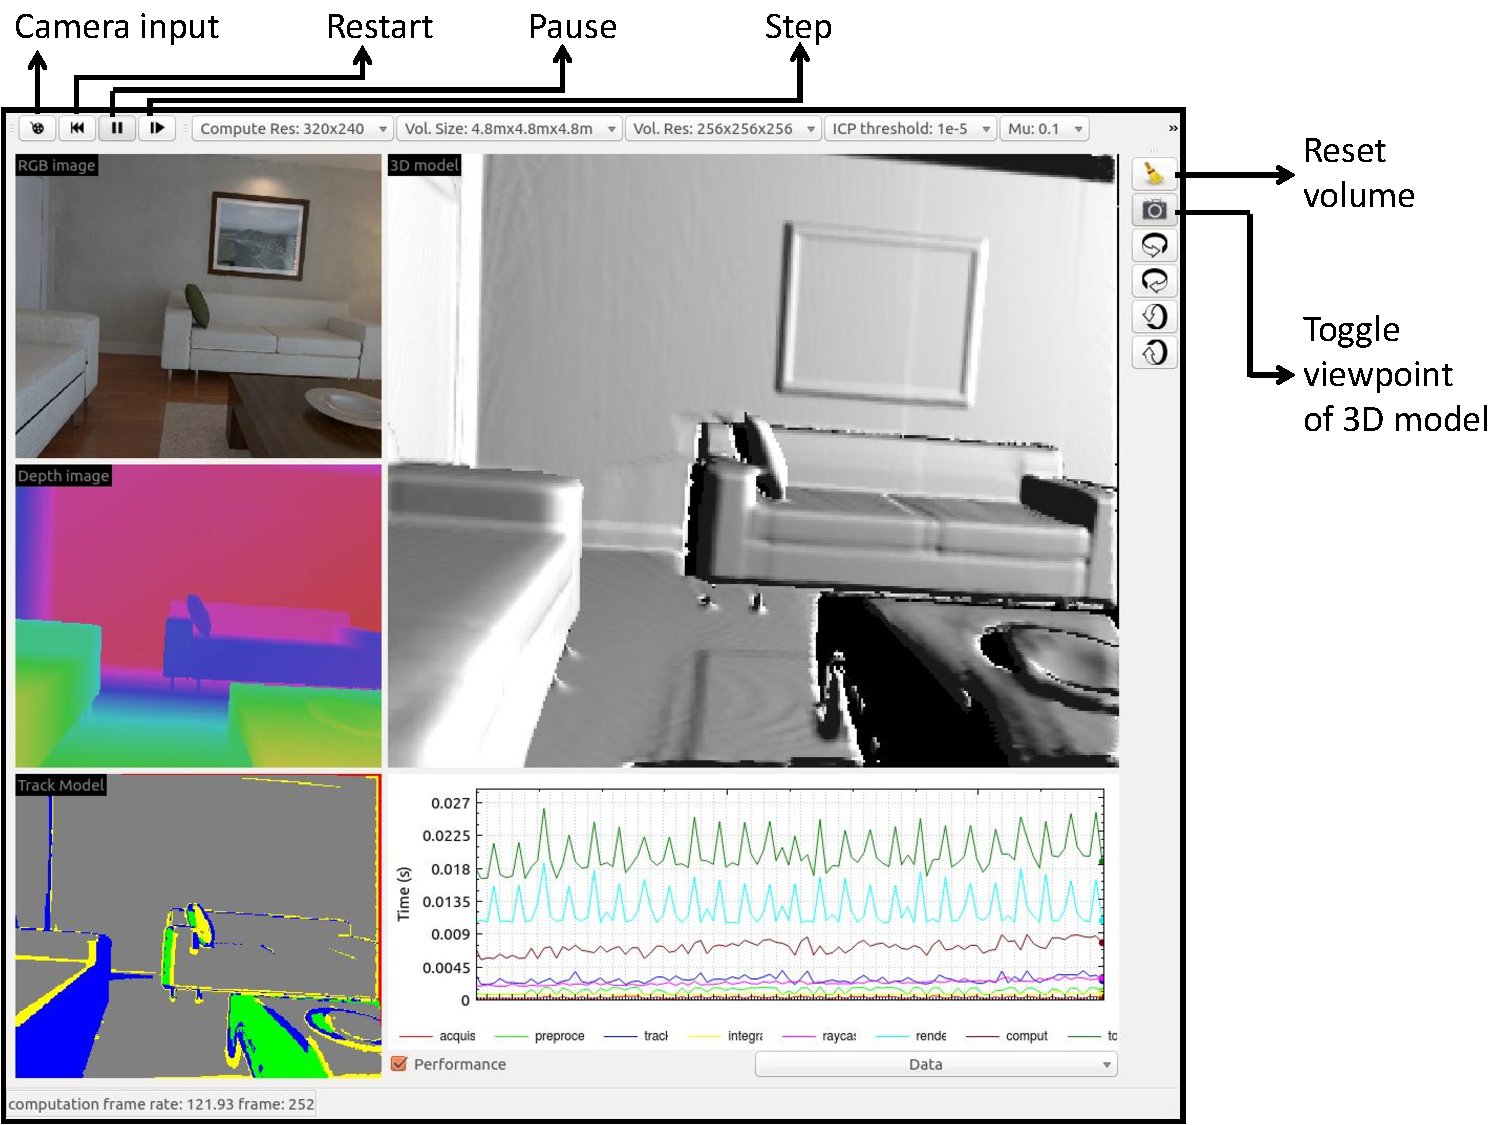
\includegraphics[width=7.0in]{SLAMBench_GUI.pdf}
    \caption{SLAMBench GUI}
    \label{gui}
\end{figure}

\section{Conclusion}
Note that the QT GUI is not available on all the supported platforms; in which case the meta build system decides to use a more primitive GUI. Please let us know if you discover any bugs in the software.

\begin{thebibliography}{9}
\bibitem{2014Nardi}
  L. Nardi, B. Bodin, M.Z. Zia, J. Mawer, A. Nisbet, P.H.J. Kelly, A.J. Davison, M. Lujan, M.F.P. O`Boyle, G. Riley, N. Topham and S. Furber.
  \emph{Introducing {SLAMBench}, a performance and accuracy benchmarking methodology for {SLAM}}.
  	arXiv:1410.2167 [cs.RO],
  2014.

\bibitem{2014Handa}
  A. Handa, T. Whelan, J.B. McDonald and A.J. Davison.
  \emph{A Benchmark for {RGB-D} Visual Odometry, {3D} Reconstruction and {SLAM}}.
  Proceedings of International Conference on Robotics and Automation (ICRA),
  2014.

\end{thebibliography}

\end{document}
